\subsection{Implementación}

Se completó \texttt{uniformCostSearch(problem)} en \texttt{pacman/search.py}. Es una búsqueda
en grafo con cola de prioridad (\texttt{util.PriorityQueue}) ordenada por $g(n)$, el costo
acumulado real desde el estado inicial. Se mantiene un diccionario con el mejor costo conocido
por estado para evitar volver a expandir un nodo cuando ya se encontró un camino más barato hacia
él (\texttt{util.PriorityQueue} no soporta \emph{decrease-key}, así que las entradas obsoletas se
descartan al extraerlas de la cola en lugar de actualizarse en el lugar).

\begin{figure}[H]
\centering
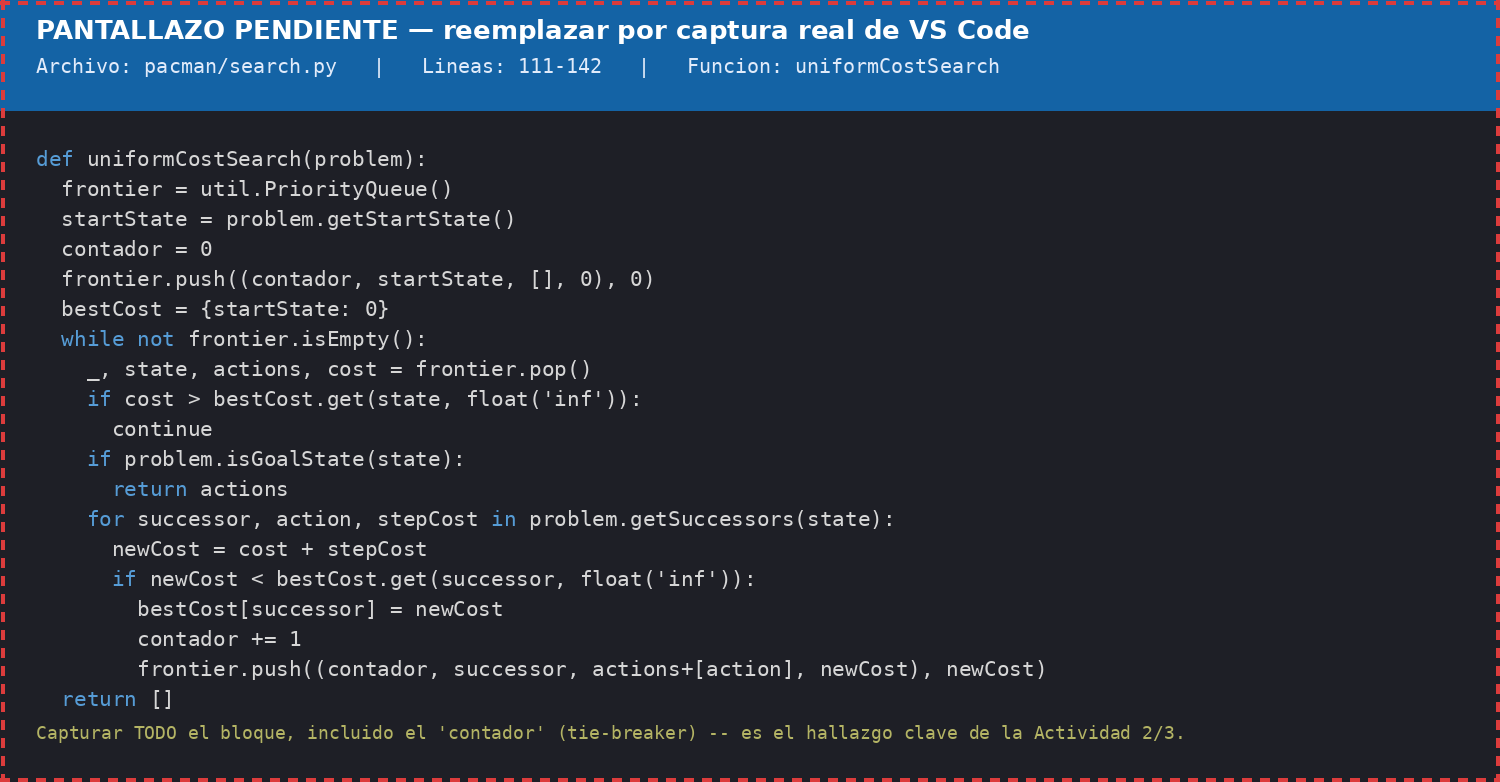
\includegraphics[width=0.95\textwidth]{capturas/actividad02_ucs.png}
\caption{Implementación de \texttt{uniformCostSearch} en \texttt{pacman/search.py} (líneas
111-142), incluido el contador de desempate \texttt{contador} explicado más abajo.}
\label{fig:act02-ucs}
\end{figure}

\subsection{Procedimiento y resultados}

Se ejecutó (ver \texttt{experimentos/actividad2\_ucs.py}) sobre \texttt{mediumMaze} y
\texttt{tinyMaze} como primera línea base.

\begin{table}[H]
\centering
\caption{Resultado de UCS (línea base para comparar A*)}
\label{tab:act2-ucs}
\begin{tabular}{lrrrr}
\toprule
\textbf{Layout} & \textbf{Costo} & \textbf{Longitud} & \textbf{Nodos expandidos} & \textbf{Tiempo (s)} \\
\midrule
mediumMaze & 30 & 30 & 32 & 0.000270 \\
tinyMaze (verificación) & 10 & 10 & 21 & 0.000182 \\
mediumClassic & 12 & 12 & 69 & 0.000492 \\
\bottomrule
\end{tabular}
\end{table}

Estos resultados se guardaron en \texttt{resultados/resultados.csv} y se usarán como línea base
para comparar A* en las Actividades 4, 6 y 9.

\subsection{Corrección de layout de referencia (detectada al verificar A* en la Actividad 3)}

Al implementar A* (Actividad 3) y compararlo contra esta línea base, se encontró que
\texttt{mediumMaze} es esencialmente un pasillo sin bifurcaciones: A* con heurística nula,
Manhattan y Euclidiana expanden exactamente los mismos 32 nodos que UCS, porque no hay ningún
punto de decisión donde una heurística pueda \emph{preferir} una dirección sobre otra. Eso hace
que \texttt{mediumMaze} no sirva para ilustrar el efecto de las heurísticas que piden las
Actividades 5, 6 y 9.

Por eso, a partir de la Actividad 3, se adopta \texttt{mediumClassic} como layout principal para
comparar UCS y A* con distintas heurísticas: tiene bifurcaciones reales y, como se muestra en la
Actividad 3, allí Manhattan sí reduce los nodos expandidos frente a UCS (69 $\rightarrow$ 15).
\texttt{mediumMaze} se conserva como caso de contraste ilustrativo (``¿qué pasa si el laberinto no
tiene bifurcaciones?''), no como el layout principal de la comparación.

\subsection{Hallazgo relevante: \texttt{python pacman.py -l mediumMaze -p SearchAgent -a fn=ucs}}

Al correr ese comando de la guía tal cual, se obtienen exactamente los mismos números
(costo, nodos expandidos y tiempo), pero el proceso termina con
\texttt{Exception: Illegal action Stop} justo después de imprimirlos. La causa no es la búsqueda:
es que los layouts de este proyecto traen muchos alimentos (no solo uno en la meta), así que al
terminarse el plan de \texttt{SearchAgent} (que la guía exige no modificar) el juego sigue
corriendo; \texttt{SearchAgent.getAction} devuelve entonces \texttt{Directions.STOP}, y en este
motor \texttt{PacmanRules.getLegalActions} elimina explícitamente \texttt{STOP} de las acciones
legales de Pac-Man. Como las métricas se calculan e imprimen dentro de
\texttt{registerInitialState}, antes de que ocurra ese error, esto no afecta ningún resultado
reportado en este informe; por eso los scripts de \texttt{experimentos/} miden directamente sobre
el \texttt{SearchProblem} en lugar de sobre el bucle completo del juego.

\subsection{Análisis}

UCS garantiza encontrar el camino de menor costo porque expande siempre el nodo de menor $g(n)$
conocido; en este problema, con costo uniforme de 1 por movimiento, eso equivale a expandir en
orden de menor número de pasos. Al no usar ninguna heurística, UCS no tiene forma de
``orientarse'' hacia el objetivo: expande por igual en todas las direcciones prometedoras según el costo
acumulado, sin preferir las que se acercan geométricamente a la meta. Esto explica por qué,
a partir de la Actividad 4, A* con una heurística informativa expandirá menos nodos que UCS para
llegar al mismo costo óptimo.
